\section{eo\-Object Class Reference}
\label{classeo_object}\index{eoObject@{eoObject}}
eo\-Object used to be the base class for the whole hierarchy, but this has changed.  


{\tt \#include $<$eo\-Object.h$>$}

Inheritance diagram for eo\-Object::\begin{figure}[H]
\begin{center}
\leavevmode
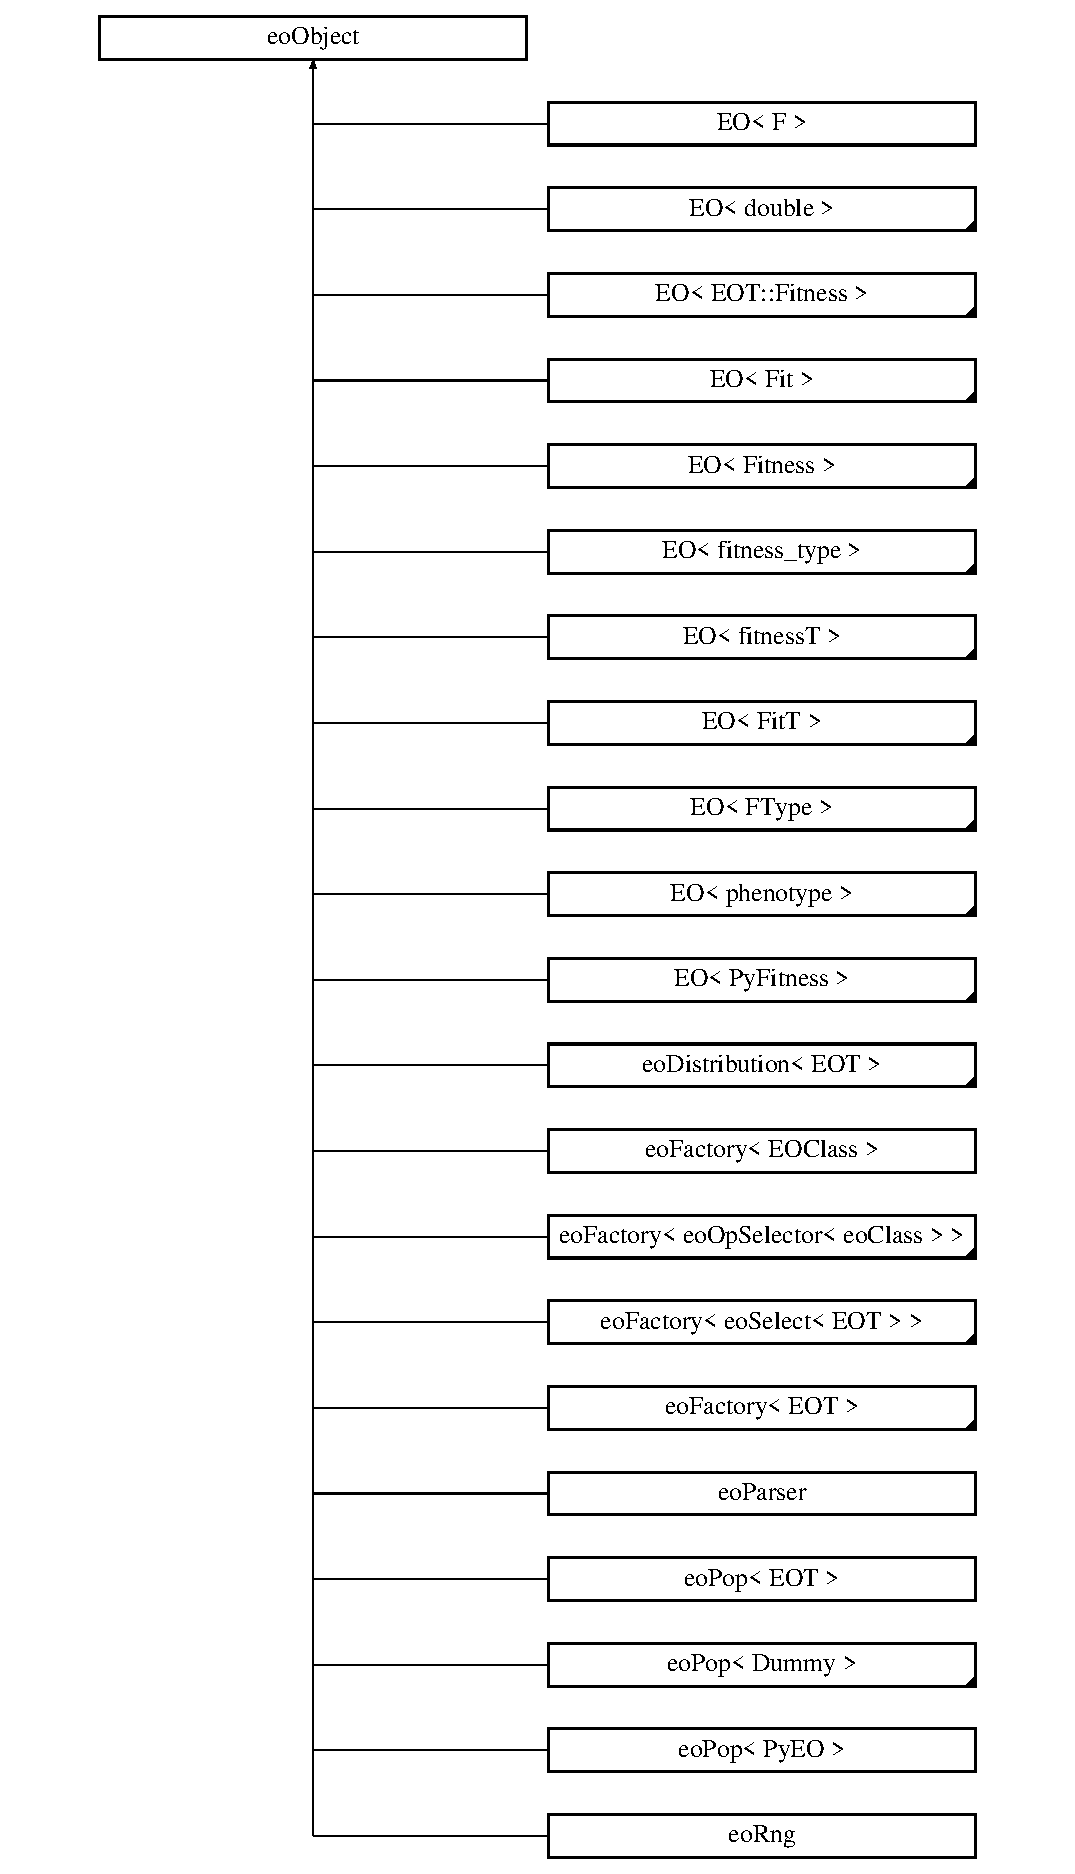
\includegraphics[height=12cm]{classeo_object}
\end{center}
\end{figure}
\subsection*{Public Member Functions}
\begin{CompactItemize}
\item 
virtual {\bf $\sim$eo\-Object} ()\label{classeo_object_a0}

\begin{CompactList}\small\item\em Virtual dtor. They are needed in virtual class hierarchies. \item\end{CompactList}\item 
virtual std::string {\bf class\-Name} () const =0
\begin{CompactList}\small\item\em Return the class id. \item\end{CompactList}\end{CompactItemize}


\subsection{Detailed Description}
eo\-Object used to be the base class for the whole hierarchy, but this has changed. 

eo\-Object is used to define a name ({\bf class\-Name}{\rm (p.\,\pageref{classeo_object_a1})}\#) that is used when loading or saving the state.

Previously, this object also defined a print and read interface, but it180s been moved to {\bf eo\-Printable}{\rm (p.\,\pageref{classeo_printable})} and {\bf eo\-Persistent}{\rm (p.\,\pageref{classeo_persistent})}.

It is recommended that you only derive from eo\-Object in concrete classes. Some parts of {\bf EO}{\rm (p.\,\pageref{class_e_o})} do not implement this yet, but that will change in the future. eo\-Object, together with {\bf eo\-Persistent}{\rm (p.\,\pageref{classeo_persistent})} and {\bf eo\-Printable}{\rm (p.\,\pageref{classeo_printable})} provide a simple persistence framework that is only needed when the classes have state that changes at runtime.

\begin{Desc}
\item[See also:]{\bf eo\-Persistent}{\rm (p.\,\pageref{classeo_persistent})} {\bf eo\-Printable}{\rm (p.\,\pageref{classeo_printable})}, {\bf eo\-State}{\rm (p.\,\pageref{classeo_state})} \end{Desc}




Definition at line 55 of file eo\-Object.h.

\subsection{Member Function Documentation}
\index{eoObject@{eo\-Object}!className@{className}}
\index{className@{className}!eoObject@{eo\-Object}}
\subsubsection{\setlength{\rightskip}{0pt plus 5cm}virtual std::string eo\-Object::class\-Name () const\hspace{0.3cm}{\tt  [pure virtual]}}\label{classeo_object_a1}


Return the class id. 

This should be redefined in each class. Only \char`\"{}leaf\char`\"{} classes can be non-virtual.

Maarten: removed the default implementation as this proved to be too error-prone: I found several classes that had a typo in class\-Name (like classname), which would print eo\-Object instead of their own. Having it pure will force the implementor to provide a name. 

Implemented in {\bf EO$<$ F $>$} {\rm (p.\,\pageref{class_e_o_z10_0})}, {\bf eo\-Factory$<$ EOClass $>$} {\rm (p.\,\pageref{classeo_factory_z13_0})}, {\bf eo\-Op\-Sel\-Mason$<$ eo\-Class $>$} {\rm (p.\,\pageref{classeo_op_sel_mason_z17_0})}, {\bf eo\-Pop$<$ EOT $>$} {\rm (p.\,\pageref{classeo_pop_z19_1})}, {\bf eo\-Es\-Full$<$ Fit $>$} {\rm (p.\,\pageref{classeo_es_full_a1})}, {\bf eo\-Es\-Simple$<$ Fit $>$} {\rm (p.\,\pageref{classeo_es_simple_a1})}, {\bf eo\-Es\-Stdev$<$ Fit $>$} {\rm (p.\,\pageref{classeo_es_stdev_a1})}, {\bf eo\-Real$<$ Fit\-T $>$} {\rm (p.\,\pageref{classeo_real_a1})}, {\bf eo\-Bit$<$ Fit\-T $>$} {\rm (p.\,\pageref{classeo_bit_a1})}, {\bf eo\-PBILDistrib$<$ EOT $>$} {\rm (p.\,\pageref{classeo_p_b_i_l_distrib_a6})}, {\bf eo\-Parse\-Tree$<$ FType, Node $>$} {\rm (p.\,\pageref{classeo_parse_tree_a4})}, {\bf eo\-String$<$ fitness\-T $>$} {\rm (p.\,\pageref{classeo_string_z26_0})}, {\bf eo\-Parser} {\rm (p.\,\pageref{classeo_parser_a4})}, {\bf eo\-Rng} {\rm (p.\,\pageref{classeo_rng_a18})}, {\bf eo\-One\-Max$<$ Fit\-T $>$} {\rm (p.\,\pageref{classeo_one_max_a2})}, {\bf EO$<$ double $>$} {\rm (p.\,\pageref{class_e_o_z10_0})}, {\bf EO$<$ EOT::Fitness $>$} {\rm (p.\,\pageref{class_e_o_z10_0})}, {\bf EO$<$ Fit\-T $>$} {\rm (p.\,\pageref{class_e_o_z10_0})}, {\bf EO$<$ phenotype $>$} {\rm (p.\,\pageref{class_e_o_z10_0})}, {\bf EO$<$ fitness\-T $>$} {\rm (p.\,\pageref{class_e_o_z10_0})}, {\bf EO$<$ Fit $>$} {\rm (p.\,\pageref{class_e_o_z10_0})}, {\bf EO$<$ FType $>$} {\rm (p.\,\pageref{class_e_o_z10_0})}, {\bf EO$<$ fitness\_\-type $>$} {\rm (p.\,\pageref{class_e_o_z10_0})}, {\bf EO$<$ Fitness $>$} {\rm (p.\,\pageref{class_e_o_z10_0})}, {\bf EO$<$ Py\-Fitness $>$} {\rm (p.\,\pageref{class_e_o_z10_0})}, {\bf eo\-Factory$<$ eo\-Op\-Selector$<$ eo\-Class $>$ $>$} {\rm (p.\,\pageref{classeo_factory_z13_0})}, {\bf eo\-Factory$<$ EOT $>$} {\rm (p.\,\pageref{classeo_factory_z13_0})}, {\bf eo\-Factory$<$ eo\-Select$<$ EOT $>$ $>$} {\rm (p.\,\pageref{classeo_factory_z13_0})}, {\bf eo\-Pop$<$ Py\-EO $>$} {\rm (p.\,\pageref{classeo_pop_z19_1})}, and {\bf eo\-Pop$<$ Dummy $>$} {\rm (p.\,\pageref{classeo_pop_z19_1})}.

The documentation for this class was generated from the following file:\begin{CompactItemize}
\item 
eo\-Object.h\end{CompactItemize}
